\textnormal{
\begin{itemize} 
\item{ The relation along with the attributes look like: }
\\Relation: Buys
\\Attributes: UName (account user name) : int, Pid (Part ID) : int, BuysID : int, Date : String
\\Relation to user scenario: This relation is to keep track of each unique purchase (BuysID) by a given user with a UName that purchases part with unique Pid at a given date.
\\Related Entities: Part, User
\\
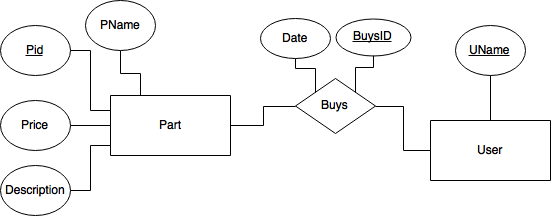
\includegraphics[width=\columnwidth]{BuysRelation.png}
\\
\\Relation: Writes
\\Attributes: Uid : int, Rid : int, Pid : int
\\Relation to user scenario: This relation occurs as described in part 1 when a account user wishes to write at most one review on a given part. Used to keep track of the Uid (user id), and Rid (review id) in relation with the Pid (part id).
\\Related Entities: Review, Account User, Part
\\
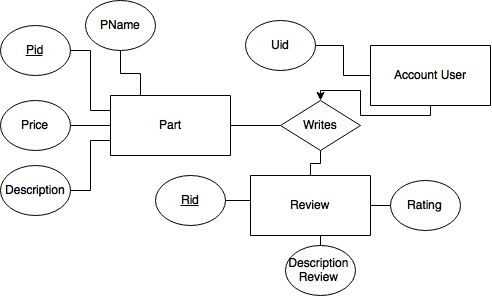
\includegraphics[width=\columnwidth]{WritesRelation.png}
\\
\\Relation: Distributes To
\\Attributes: Cid (Company id) : int, Sid (Seller id) : int
Relation to user scenario: When a user wishes to buy a part, they are given a link to the sellers which distribute the part, in order for them to distribute to the users, companies must first distribute the part to each seller. Each company distributes their part to atleast one seller to then sell that part.
\\Related Entities: Company, Seller
\\
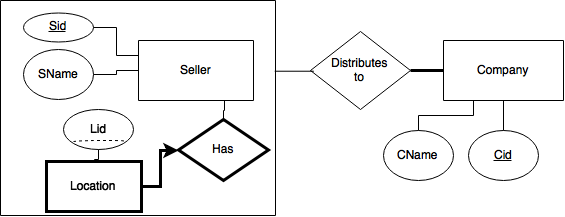
\includegraphics[width=\columnwidth]{distributesrelation.png}
\\
\\Relation: Sold By
\\Attributes: Sid : int, Pid : int
\\Relation to user scenario: Similar to the previous scenario, when an account user makes a purchase they are given a link to the seller of their choosing. This relation relates all sellers to products they sell, and all sellers who sell a certain part. 
\\Related Entities: Seller, Part
\\
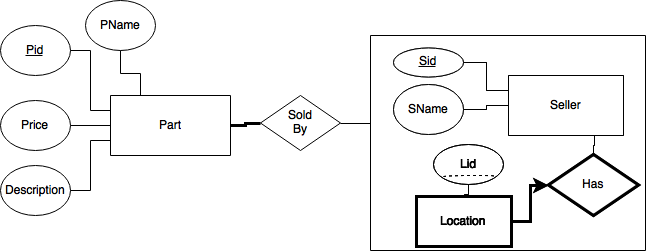
\includegraphics[width=\columnwidth]{soldbyrelation.png}
\\
\\Relation: Manufactures
\\Attributes: Pid : int, Cid : int
\\Relation to user scenario: When a company releases a new part, this relation keeps track of how each part is manufactured. Each individual product in the Computer Hardware Database is manufactured by exactly one company. For example: Intel and Kingston cannot both manufacture Intel Core i7 Processors, only Intel can.
\\Related Entities: Part, Company
\\
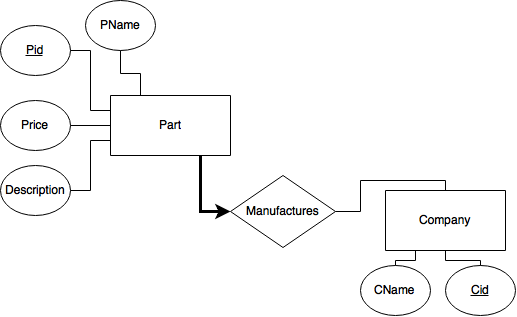
\includegraphics[width=\columnwidth]{manufacturesrelation.png}
\\
\\Relation: Has
\\Attributes: Lid : int, Sid : int
\\Relation to user scenario: When describing the Seller entity, we decided to describe it in terms of an additional relation and entity within an aggregate. Whenever a seller is called upon within a relation, the seller location will describe that seller within a unique location containing a Lid. This relation is a weak entity in that if a Seller is removed, the location describing that seller will be removed as well.
\\
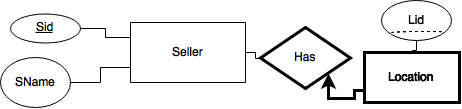
\includegraphics[width=\columnwidth]{residesrelation.png}
\\
\\Relation: Reviews
\\Attributes: Rid : int, Pid : int
\\Relation to user scenario: Each review reviews exactly 1 part. This relation keeps track of the review id and the part that it applies to. 
\\Related Entities: Part, Review
\\
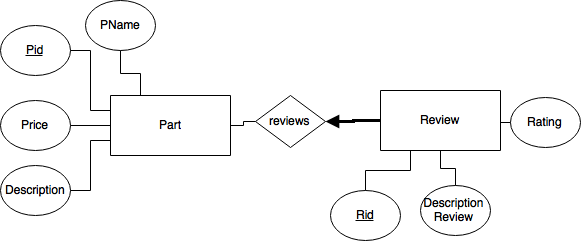
\includegraphics[width=\columnwidth]{hasrelation.png}
\\
\\Relation: is Part of
\\Attributes: Pid1 : int, Pid2 : int
\\Relation to user scenario: Each part is a component of multiple parts. In a real-world user scenario, computer parts are very complex and made up of multiple individual computer parts. We accounted for this by implementing this relation.
\\Related Entities: Part
\\
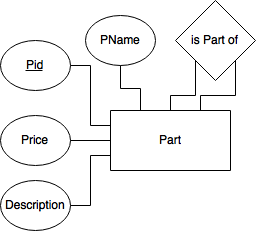
\includegraphics[width=\columnwidth]{ispartofrelation.png}
\\
\item{ The description relating this ER part (relation) as it corresponds to one or more user scenario(s): }
Please insert the description relating this ER part to user scenario(s), in here.
\end{itemize}
Please repeat that pattern for each relation.
\begin{itemize} 
\item{ The ER diagram in its entirety: }
\\
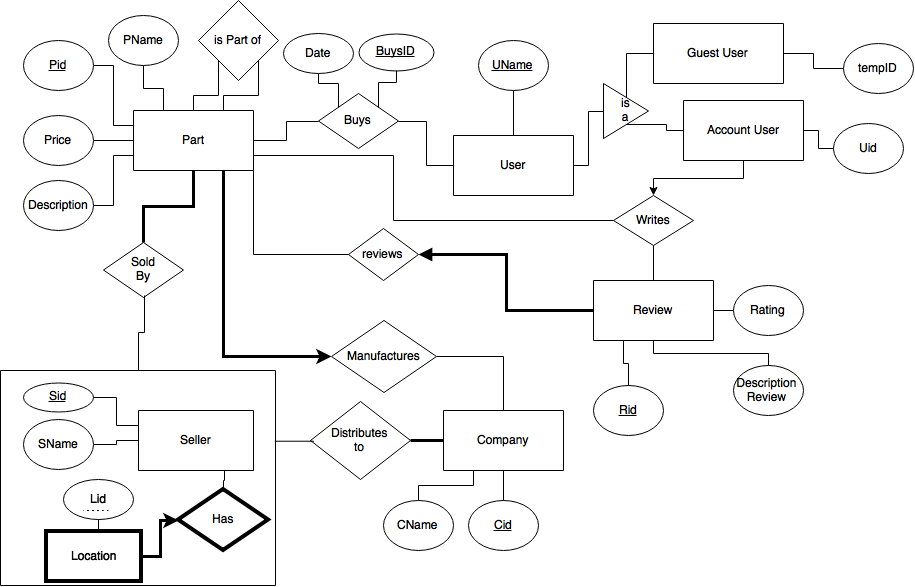
\includegraphics[width=\columnwidth]{ERDiagram.png}
\item{ The ER diagram description (corresponding to the user scenarios): }
Above is our ER diagram depicting numerous user type scenarios that could take place within our computer hardware database. In our ER diagram, we based the different user types as entities themselves, with the addition of a ''Review'' and ''Part'' entity. Having user types as entities allows us leeway for enacting our user scenarios through the use of relations of those entities. The ER diagram closely follows the user scenarios that were previously described in this report. For example, the ''User'' entity ''Buys'' a ''Part'' that is ''Sold By'' a ''Seller''. This scenario is clearly depicted in the ER diagram above and numerous other user scenarios are clearly described as well. With the addition of the entities are their potential attributes and relations to other entities. The ''Writes'' relation relates to a ''Review'' entity and a ''Account User'' entity. The ''Part'' entity is tied to six potential relations, which includes ''Buys'',''Has'', 'Manufactures'', ''is Part of'', ''Writes'' and ''Sold Buy''. Furthermore, a ''Account User'' has the ability to ''Write'' a ''Review'' or ''Buy'' a ''Part''. Lastly, our ''Company'' entity has a primary purpose of ''Distributing to'' the ''Seller'' entity, from whom a ''Part'' is ''Sold by''. In regards to the attributes we have chosen for each entity, all entities contain at least one primary key that helps to distinguish themselves from other entities. Overall, we tried to compose a database design that was easy to follow yet completes its task quickly and without problems. All user scenarios are clearly described in this single ER diagram in such a way that connects each of our entities in a logical and reasonable manner.
\\
\item{ The integrity constraints defined in the ER diagram: }
Each part is sold by atleast one seller, each company distributes to atleast one seller that resides at a particular location, each part is manufactured by exactly one company, a covering constraint indicating that each user type must either be an ''Account User'' or a ''Guest User'', a weak entity amongst a ''Location'' that only exists if there is a ''Seller'' entity and each account user writes at most one review for a given part. Additionally, each ''Review'' ''reviews'' exactly one ''Part''. 
\begin{itemize} 
\item{ Integrity Constraint: }
Each part is sold by at least one seller.
\item{ The description and justification of the integrity constraint: }
The first integrity constraint we included in our ER diagram relates to the ''Part'' entity and the ''Sold By'' relation. In order to make logical sense of our ER diagram, we created this constraint with the fact that  a part is sold by atleast one seller. A single part can be sold by multiple sellers. 
\end{itemize}
\begin{itemize} 
\item{ Integrity Constraint: }
Each company distributes to at least one seller that resides in a location (aggregate).
\item{ The description and justification of the integrity constraint: }
The second integrity constraint we included in our ER diagram relates to the ''Company'' entity and the ''Distributes to'' relation. We constructed this constraint with the idea that at a Company distributes their manufactured part to atleast one ''Seller''. A  company should be able to distribute their part to a collection of sellers. 
\end{itemize}
\begin{itemize} 
\item{ Integrity Constraint: }
Each part is manufactured by exactly one company.
\item{ The description and justification of the integrity constraint: }
The third integrity constraint we included in our ER diagram relates to the ''Part'' entity and the ''Manufactures'' relation to ''Company'. Each part in the database is manufactured by exactly one company. No identical part is manufactured by more than one company. Each company can manufacture many parts as well.
\end{itemize}
\begin{itemize} 
\item{ Integrity Constraint: }
A covering constraint indicating that each user type must either be an ''Account User'' or a ''Guest User''
\item{ The description and justification of the integrity constraint: }
In our model, we have two potential user types that have similar roles but vary in allowed attributes. As compared to account users who carry a unique Uid, guest users carry a tempID that distinguishes them from account users. By implementing an ISA relationship, we can account for both account users and guest users.
\end{itemize}
\begin{itemize} 
\item{ Integrity Constraint: }
A weak entity amongst a ''Location''. Each seller location only exists if there is a ''Seller'' entity. 
\item{ The description and justification of the integrity constraint: }
In order for there to be a seller location, a seller must exist. This indicates that the ''Location'' entity is a weak entity in the fact that a location can not exist without a seller. Each location has a seller tied to it and will be deleted if a seller is deleted from the database.  
\end{itemize}
\begin{itemize} 
\item{ Integrity Constraint: }
Each Account User writes at most one review for a given part.
\item{ The description and justification of the integrity constraint: }
In our computer hardware database design, we decided that an account user type can write a single review on a give computer part. To account for this, we drew an arrow relating the ''Review'' and ''Writes'' relationship in order to indicate this constraint. An account user should not be able to write multiple reviews on a single computer hardware part. This keeps the database free from user-review spamming and keeps the integrity of the content in our database at a high level. 
\end{itemize}
\end{itemize}
}
